\section{Interfejs MPI}

\subsection{Model sieciowy}

Komunikacja odbywa sie za pomocą przesyłania wiadomości (czyli między innymi w standardzie MPI) w tak zwanym modelu sieciowym. Składa się on z określonej liczby procesorów, przy czym każdy z nich posiada własną pamięć lokalną. Procesory posiadają dostęp jedynie do instrukcji i danych przechowywanych w swojej pamięci lokalnej -- nie istnieje pamięć wspólna. Aby umożliwić wymianę informacji pomiędzy procesorami, tworzona jest sieć połączeń (ang \textit{interconnection network}), która zbudowana jest z dwukierunkowych kanałów komunikacyjnych (łącz). 

\begin{figure}[h]
	\centering
	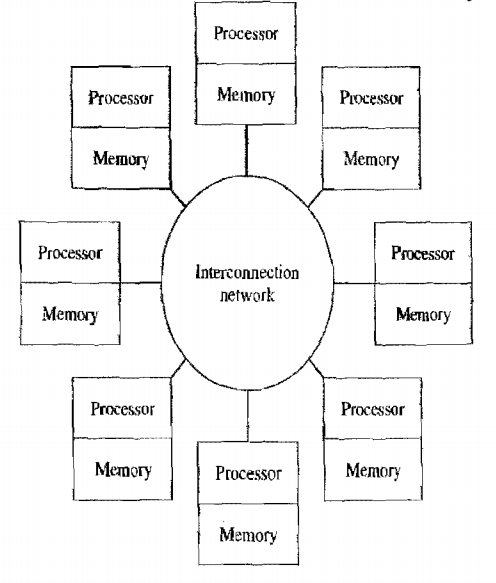
\includegraphics[width=0.85\textwidth]{./img/sieciowy.png}
	\caption{Model sieciowy. Źródło: \cite{Parallel}, str 94}
	\label{img:sieć}
\end{figure}

Wymiana informacji między procesorami jest realizowana poprzez kooperujące ze sobą procedury trasowania (ang. \textit{routing}), które działają w każdym procesorze. Dzięki nim, każdy węzeł sieci (tutaj: procesor) posiada informację, z którymi węzłami może wymieniać informacje. Zbiór wszystkich procedur trasowania definiuje \textbf{topologię sieci połączeń}. Można ją opisać przy pomocy grafu, gdzie wierzchołkami (węzłami) są procesory, natomiast krawędzi to dwukierunkowe łącza.

Ocenę skuteczności/przydatności danej sieci podczas prowadzenia obliczeń równoległych można określić biorąc pod uwagę kilka parametrów:

\begin{itemize}
	\item \textbf{Średnica sieci} (ang \textit{diameter}) -- maksymalna odległość zmierzona za pomocą liczby krawędzi między dowolnymi dwoma wierzchołkami. Im mniejsza średnica, tym lepsza jest sieć -- oznacza to, że informacje będą potrzebowały średnio mniej czasu na dotarcie do właściwego odbiorcy. Przypadek pesymistyczny zakłada, że wiadomość będzie musiała zostać przesłana przez liczbę krawędzi równej średnicy.
	\item \textbf{Szerokość połowienia sieci} (ang. \textit{bisection width}) -- minimalna liczba krawędzi, którą należy usunąć z obecnej sieci, aby móc ją podzielić na 2 równe podsieci.
	\item \textbf{Szerokość pasma} (ang. \textit{bisection bandwidth}) -- jest to iloczyn szerokości połowienia oraz szybkości przesyłu danych w pojedynczym kanale. Pozwala określić liczbę bitów, jaką można przesłać między podsieciami w jednostce czasu. Im większa szerokość pasma, tym lepiej.
	\item \textbf{Maksymalny stopień wierzchołka} -- maksymalna liczba krawędzi połączonych z danym wierzchołkiem (liczona globalnie dla całej sieci). Dla niewielkiego stopnia łatwiej zaprogramować procedury komunikacyjne ze względu na fakt, że używają one mniejszej liczby kanałów. Zakłada się, że sieć jest dobra jeżeli przy wzroście liczby p procesorów średnica sieci rośnie nie szybciej niż logarytmicznie w funkcji p, natomiast maksymalny stopień wierzchołka jest stałą liczbą o małej wartości.
	\item \textbf{Spójność krawędziowa} (ang. \textit{edge connectivity}) -- definiowana jaka minimalna liczba krawędzi, które muszą zostać wyłączone z sieci aby ta stała się niespójna (graf rozłoży się na 2 lub więcej osobnych podgrafów). Im większa spójność krawędziowa, tym odporniejsza jest sieć -- istnieje mniejsze prawdopodobieństwo całkowitego unieruchomienia sieci w przypadku, gdy któryś procesor ulegnie uszkodzeniu. Większa spójność prowadzi też do zmniejszenia rywalizacji poszczególnych węzłów o łącze.
	\item \textbf{Koszt sieci} -- zazwyczaj określana jako suma wszystkich kanałów w sieci.
\end{itemize}

Przykładowe topologie sieci połączeń:

\begin{itemize}
	\item siatka
	\item torus (jedno-, wielowymiarowy)
	\item kostka (jedno-, wielowymiarowa)
\end{itemize}

\begin{figure}[h]
	\centering
	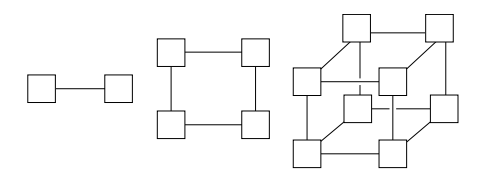
\includegraphics[width=0.85\textwidth]{./img/kostki.png}
	\caption{Topologia kostki. Od lewej: jedno-, dwu- oraz trójwymiarowa. Źródło: \cite{Pacheco}, str 40}
	\label{img:sieć}
\end{figure}

\subsection{Zasada działania MPI}

MPI jako interfejs przeznaczony do pracy z obliczeniami rozproszonymi oparty został o model sieciowy, posiadaja jednak kilka cech, które wyróżniają od standardowej implementacji tego wzorca. MPI można potraktować jako interfejs pomiędzy programem a systemem operacyjnym.

Tradycyjnie, każdy z procesów posiada własną pamięć lokalną, co narzuca konieczność komunikacji przez dwukierunkowe łącza kounikacyjne (w nomenklaturze MPI nazwywane \textbf{komunikatorami}). Komunikacja polega na przesłaniu danych z pamięci procesu źródłowego do pamięci lokalnej procesu docelowego przy wykorzystaniu węzłów pośrednich. Domyślnie każdy nowoutworzony proces znajduje się w komunikatorze świat (MPI\textunderscore COMM\textunderscore WORLD). Takie rozwiązanie sprawia, że każdy proces może wymieniać dane z dowolnym pośród pozostałych, niezależnie od fizycznej struktury procesorów (jest ona przezroczysta dla procesów). Istnieje możliwość zdefiniowania własnych komunikatorów -- co może okazać się przydatne w przypadku, gdy programista chce zawężyć zakres procesów, do których wysyłana jest wiadomość rozgłoszeniowa (ang. \textit{broadcast}).

W trakcie tworzenia programu w oparciu o ten interfejs, warto podzielić część programu przeznaczoną do obliczeń rozproszonych na części, które mają zostać przydzielone do osobnych procesów. Na początku pracy, deklarowana jest ilość procesów, które mają zostać zaangażowane do pracy. Może się to odbywać na jeden z 2 sposobów:

\begin{itemize}
	\item Statyczny -- procesy tworzone są przed wykonaniem programu. Program (proces główny, tak zwany \textit{root}) nie może zostać zakończony przed końcem pracy wszystkich pozostałych procesów.
	\item Dynamiczny -- Potrzebne procesy są tworzone podczas pracy programu. Ta opcja jest dostępna wyłącznie dla wersji MPI-2 (zaprezentowanej w 1997 roku).
\end{itemize}

Każdy utworzony proces posiada własny unikalny identyfikator (id) w ramach komunikatora. W różnych komunikatorach ten sam proces może posiadać różne id. Identyfikatorem procesu głównego (\textit{roota}) jest liczba 0.

W momencie tworzenia nowego procesu, tworzona jest kopia programu przeznaczonego tylko dla tego procesu. W praktyce oznacza to, że posiada dostęp do każdej zmiennej zadeklarowanej globalnie, jednak tylko w ramach lokalnej kopii. W przypadku, gdy proces potrzebuje danych znajdujących się w innym węźle, konieczna jest wymiana informacji w ramach komunikatora. Do rozdzielania pracy stosuje się standardowe operacje rozgałęzienia (między innymi instrukcje \textit{if} czy \textit{else} w językach C/C++) identyfikując id procesu. Jest to technika zwana SPMD (\textit{Single Program Multiple Data} -- pojedynczy program, wiele danych), będący subkategorią MIMD (\textit{Multiple Instruction Multiple Data} - wiele instrukcji, wiele danych), znanej z taksonomii Flynna. Zazwyczaj utworzone kopie programów działają w sposób asynchroniczny, lecz może dojść do sytuacji, w której procesy te będą działały synchronicznie. Określony sposób działania może być uzależniony od funkcji, jakie zostaną użyte przez programistę.

\subsection{Kompilacja i uruchamianie}

Szczegóły związane z kompilacją i uruchamianiem programu napisanego przy użyciu biblioteki MPI są zależne od używanego systemu operacyjnego. Większość z nich do kompilacji używa komendy, której można użyć z poziomu linii poleceń/terminala: \\

\texttt{\$ mpicc -o <plik\textunderscore źródłowy> <plik\textunderscore wynikowy>.c} \\

Zazwyczaj \texttt{mpicc} jest skryptem opakowującym (ang. \textit{wrapper script}) dla kompilatora języka (dla powyższego przypadku, języka C). Skrypt opakowujący jest pisany w celu uruchomienia określonego programu. Skrypt ten upraszcza uruchomienie kompilatora poprzez jawne wskazanie, w którym miejscu znajdują się potrzebne pliki nagłówkowe oraz które biblioteki należy połączyć z plikiem obiektu.

Uruchamianie skompilowanego programu odbywa się przez następującą komendę: \\

\texttt{mpirun -np <liczba\textunderscore procesów> <nazwa\textunderscore pliku\textunderscore wynikowego> <parametry>} \\

W wyżej wymienionej komendzie '\texttt{liczba\textunderscore procesów} jest liczbą całkowitą dodatnią i wskazuje, ile procesów ma być wykonanych równolegle. \texttt{nazwa\textunderscore pliku\textunderscore wynikowego} oraz \texttt{parametry} przekazywane są do procesów za pośrednicztwem zmiennych \texttt{argc} i \texttt{argv} znajdujących się w nagłówku funkcji main (zgodnie z zasadami języka C).


\subsection{Inicjalizacja i kończenie programu}

Większość elementów składowych programu napisanego przy użyciu MPI jest instrukcjami natywnymi używanego języka (C, C++, Ada, Fortran). Aby umożliwić korzystanie z instrukcji nowej biblioteki, należy dodać następującą instrukcję (przykład dla języka C): \\

\texttt{include "mpi.h"} \\

Spowoduje to włączenie pliku nagłówkowego \texttt{mpi.h}. Znajdują się w nim prototypy funkcji MPI, makrodefinicje, definicje typów oraz inne  definicje i deklaracje potrzebne do skompilowania programu MPI. Pierwszą instrukcją, jaka jest wykonywana przed rozdzieleniem pracy pomiędzy wątki jest \texttt{MPI\textunderscore INIT} o następującej składni: \\

\begin{lstlisting}[language=C]
int MPI_Init(
	int* argc_p 
	char*** argv_p)
\end{lstlisting} 

Argumenty funkcji są wskaźnikami do argumentów funkcji main, kolejno \texttt{argc} i \texttt{argv}. W przypadku, gdy parametry wywołania nie istnieją lub nie są potrzebne dla instrukcji MPI, można do obu przekazać wartość NULL. Wartością zwracaną przez \texttt{MPI\textunderscore Init} jest kod błędu, co jest standardem dla większości funkcji tej biblioteki. Jeżeli zwrócona wartość jest równa \texttt{MPI\textunderscore SUCCESS}, oznacza to poprawne wykonanie inicjalizacji. Pozostałe kody oznaczają błędy jakie wystąpiły podczas pracy, a ich wartości uzależnione są od implementacji bilioteki. Informację o tym, czy w danym momencie programu mechanizm MPI został zainicjalizowany, możemy uzyskać za pomocą funkcji \texttt{MPI\textunderscore Initialized}. Rzadziej używaną alternatywą dla \texttt{MPI\textunderscore Init} stanowi \texttt{MPI\textunderscore Init\textunderscore thread}, który dodatkowo inicjalizuje środowisko wątków.

Analogicznie, ostatnią instrukcją, jaka powinna zostać wywołana w programie MPI, jest funkcja finalizacji: \\

\texttt{int MPI\textunderscore Finalize(void);} \\

Jej wywołanie powoduje zwolnienie wszystkich zasobów komputera, które zostały wcześniej zaalokowane przez funkcję inicjalizacji, a następnie wykorzystywane w trakcie obliczeń równoległych. Podobnie jak wcześniejsza funkcja, \texttt{MPI\textunderscore Finalize} zwraca kod błędu.

Nieobowiązkowymi, ale niemal równie ważnymi funkcjami są \texttt{MPI\textunderscore Comm\textunderscore size} oraz \texttt{MPI\textunderscore Comm\textunderscore rank} o następującej składni:

\begin{lstlisting}[language=C]
int MPI_Comm_size(
	MPI_Comm comm,
	int* comm_number);

int MPI_Comm_rank(
	MPI_Comm comm,
	int* my_rank_p);
\end{lstlisting}
 
 W obu przypadkach, pierwszym argumentem jest komunikator, w którym znajduje się proces go wywołujący. Komunikatory w bibliotece MPI są nieprzeźroczystym obiektem (tzn. o nieznanej wewnętrznej strukturze), w ramach której kolekcja procesów może wymieniać między sobą dane. Posiadają one własny typ, \texttt{MPI\textunderscore Comm}. \texttt{MPI\textunderscore Comm\textunderscore size} jako swój drugi argument zwraca liczbę procesów znajdującą się w komuikatorze, natomiast \texttt{MPI\textunderscore Comm\textunderscore rank} informuje jaki identyfikator został przydzielony procesowi który wykonał tę funkcję w ramach komunikatora. Funkcje te ułatwiają rozdzielanie zadań pomiędzy procesy oraz kontrolę nad przepływem pracy algorytmu równoległego.
 
\subsection{Typy danych w MPI}

Interfejs MPI wykorzystuje własne typy danych w trakcie wymiany informacji. Zamiast informacji o ilości przesyłanych bajtów, w trakcie transferu wysyłana jest informacja o ilości przesyłanych elementów danego typu (argument \texttt{count}). Wartość ta może być równa zero, co jest tożsame z informacją, że część wiadomości zawierająca dane jest pusta. Podstawowe typy danych MPI, których można użyć w trakcie komunikacji odpowiadają typom podstawowym języka programowania, z którego korzystamy i różnią się w zależności od implementacji.



\begin{figure}[h]
	\begin{center}
	\begin{tabular}{|c|c|}
		\hline Typ MPI & Odpowiednik w języku C \\ 
		\hline MPI\textunderscore CHAR & char \\ 
		\hline MPI\textunderscore SHORT & signed short int \\ 
		\hline MPI\textunderscore INT & signed int \\ 
		\hline MPI\textunderscore LONG & signed long int \\ 
		\hline MPI\textunderscore LONG\textunderscore LONG\textunderscore INT & signed long long int \\ 
		\hline MPI\textunderscore SIGNED\textunderscore CHAR & signed char \\ 
		\hline MPI\textunderscore UNSIGNED\textunderscore CHAR & unsigned char \\ 
		\hline MPI\textunderscore UNSIGNED & unsigned short int \\ 
		\hline MPI\textunderscore UNSIGNED\textunderscore LONG & unsigned long int \\ 
		\hline MPI\textunderscore FLOAT & float \\ 
		\hline MPI\textunderscore DOUBLE & double \\ 
		\hline MPI\textunderscore LONG\textunderscore DOUBLE & long double \\ 
		\hline MPI\textunderscore C\textunderscore BOOL & \textunderscore Bool \\ 
		\hline MPI\textunderscore BYTE & 8 bitów (8 cyfr binarnych) \\ 
		\hline MPI\textunderscore PACKED & - \\
		\hline 
	\end{tabular} 
	\captionof{table}{Najważniejsze typy MPI i ich odpowiedniki dla języka C Źródło: \cite{MPI}, str 26} \label{table:datatypes} 
	\end{center}
\end{figure}

\section{Komunikacja między procesami w biliotece MPI}

\subsection{Komunikacja punkt-punkt}

\subsubsection{MPI\textunderscore Send}
Ten rodzaj komunikacji stanowi jeden z dwóch podstawowych odmian transferu danych w modelu sieciowym. Polega on na przesyłaniu wiadomości pomiędzy określoną parą procesów. W bibliotece MPI służy do tego para funkcji \texttt{MPI\textunderscore Send} oraz \texttt{MPI\textunderscore Receive}. Składnia nagłówka pierwszej z nich prezentuje się następująco: 
\begin{lstlisting}[language=C]
int MPI_Send(
	void* message_buff,
	int message_size,
	MPI_Datatype message_type,
	int dest,
	int tag,
	MPI_Comm communicator);
\end{lstlisting}

Gdzie:
\begin{itemize}
	\item \texttt{\textbf{message\textunderscore buff}} -- pierwszy argument funkcji będący wskaźnikiem na bufor, w którym przetrzymywana jest wiadomość wysyłana przez proces. Jest to adres (w pamięci przeznaczonej na zmienne), pod którym zapisana jest wiadomość przed wysłaniem.
	\item \texttt{\textbf{message\textunderscore size}} -- określa, ile elementów ma zostać przesłanych w wiadomości.
	\item \texttt{\textbf{message\textunderscore type}} -- typ wysyłanych danych. Stanowi jeden z wbudowanych typów danych dla MPI \hyperref[table:datatypes]{Rozdział 2.5} lub typ pochodny zdefiniowany przez użytkownika.
	\item \texttt{\textbf{dest}} -- id procesu, do którego wiadomość ma zostać przesłana.
	\item \texttt{\textbf{tag}} -- liczba nieujemna z zakresu 0 do 32767 (lub więcej, zależnie od implementacji). Informacja, mająca na celu ułatwienie rozróżniania procesów. Umożliwia to wysyłanie dodatkowej informacji do innych procesów.
	\item \texttt{\textbf{communicator}} -- nazwa komunikatora, w ramach którego wysyłana jest wiadomość.
\end{itemize}

Wszystkie wymienione parametry są parametrami wejściowymi. Działanie \texttt{MPI\textunderscore Send} może być uzależnione od implementacji. Rozróżnia się 2 sposoby komunikacji:

\begin{itemize}
	\item Komunikacja synchroniczna -- polega na wstrzymaniu obliczeń przez proces wysyłający do momentu, gdy proces odbierający zgłosi gotowość do przyjęcia wiadomości. Dopiero po zgłoszeniu, informacja zostaje wysłana i procesy kontynuują pracę.
	\item Komunikacja buforowana -- po wywołaniu funkcji \texttt{MPI\textunderscore Send} wiadomość kopiowana jest do bufora, a proces wysyłający kontynuuje pracę. Proces odbierający może pobrać wiadomość z bufora w dowolnym momencie, o ile jest ona aktualnie dostępna. Ten sposób przyspiesza działanie programu w porównaniu do poprzednika, ale wymaga obecności buforowania w systemie obliczeniowym.
\end{itemize}

\subsubsection{MPI\textunderscore Receive}
Funkcją służącą do odbierania wiadomości wysłanych przy pomocy \texttt{MPI\textunderscore Send} jest \texttt{MPI\textunderscore Receive} o nagłówku:
\begin{lstlisting}[language=C]
int MPI_Recv(
	void* message_buff,
	int message_size,
	MPIDatatype message_type,
	int source,
	int tag,
	MPI_Comm communicator,
	MPI_Status* status);
\end{lstlisting}

Gdzie:

\begin{itemize}
	\item \texttt{\textbf{message\textunderscore buff}} wskazuje na obszar pamięci, do którego zapisane zostaną otrzymane dane.
	\item \texttt{\textbf{message\textunderscore size}} -- liczba danych, z których ma się składać wczytana wiadomość.
	\item \texttt{\textbf{message\textunderscore type}} -- typ wysyłanych danych. Stanowi jeden z wbudowanych typów danych dla MPI \hyperref[table:datatypes]{Rozdział 2.5} lub typ pochodny zdefiniowany przez użytkownika. Należy zwrócić szczególną uwagę, aby w obszarze pamięci, do którego będzie zapisywana wiadomość, istniała odpowiednia ilość wolnego miejsca.
	\item \texttt{\textbf{source}} -- identyfikator procesu, od którego odbierana będzie wiadomość.
	\item \texttt{\textbf{tag}} -- liczba nieujemna z zakresu 0 do 32767 (lub więcej, zależnie od implementacji). Informacja, mająca na celu ułatwienie rozróżniania procesów. Umożliwia to wysyłanie dodatkowej informacji do innych procesów.
	\item \texttt{\textbf{communicator}} -- nazwa komunikatora, w ramach którego wysyłana jest wiadomość.
	\item \texttt{\textbf{status}} -- wskaźnik do struktury przechowujacej informacje o odebranej wiadomości. Struktura taka zawiera m. in. dane o numerze (id) nadawcy, znaczniku oraz o kodzie błędu.
\end{itemize}

Większość parametrów ma charakter wejściowy, za wyjątkiem \texttt{message\textunderscore buff} oraz \texttt{status}, które mają charakter wyjściowy. Funkcja MPI\textunderscore Receive jest funkcją blokującą, co oznacza że proces w momencie jej wywołania jest blokowany do momentu odebrania wiadomości.

\subsubsection{Dodatkowe funkcje i struktury}

Dla zwiększenia elastyczności (oraz przyspieszenia wykonania programów równoległych) w bibliotece MPI zaimplementowano dodatkowe elementy:

\begin{itemize}
	\item \texttt{MPI\textunderscore ISend} -- specyficzna odmiana funkcji \texttt{MPI\textunderscore Send}. W przeciwieństwie do poprzedniczki nie blokuje procesu wysyłającego, niezależnie od obecności buforowania w systemie. Wiadomość jest wysyłana, a sterowanie natychmiast oddawane jest do procesu nadawcy, pozwalając na kontynuowanie obliczeń. Proces ten powinien po jakimś czasie wywołać funkcję \texttt{MPI\textunderscore Wait} w celu sprawdzenia, czy wysyłanie zostało zakończone.
	\item \texttt{MPI\textunderscore IReceive} -- nieblokująca odmiana
	\texttt{MPI\textunderscore Receive}. Jej wywołanie inicjuje odbieranie wiadomości, po czym sterowanie wraca do procesu wywołującego, który kontunuuje obliczenia. Podobnie jak wyżej, można wywołać funkcję \texttt{MPI\textunderscore Wait} (lub alternatywnie \texttt{MPI\textunderscore Test}) sprawdzającą, czy wiadomość została odebrana.
	\item \texttt{MPI\textunderscore ANY\textunderscore SOURCE} -- zezwala na przyjęcie danych ze dowolnego źródła.
	\item \texttt{MPI\textunderscore ANY\textunderscore TAG} -- pozwala na przyjęcie dowolnego znacznika ze źródła.
	\item \texttt{MPI\textunderscore Probe} -- funkcja pozwalająca na sprawdzenie przychodzącej wiadomości bez jej właściwego odebrania. Umożliwia uniknięcie sytuacji, w której typ oraz identyfikator nadawcy są zgodne, jednak wiadomość jest za duża i trzeba zaalokować dodatkową pamięć przed jej odebraniem.
	
\end{itemize}

\subsection{Komunikacja kolektywna oraz redukcja danych}

Komunikacja typu punkt-punkt pozwala precyzyjnie wskazać, jak ma odbywać się transfer wiadomości między procesami, nie jest jednak pozbawiony wad. W przypadku, gdy istnieje potrzeba zaangażowania dużej ilości procesów (gdzie dla nowoczesnych superkomputerów wartość ta może figurować na poziomie dziesiątek lub setek tysięcy) zaprogramowanie każdej pary procesorów między którymi ma odbywać się komunikacja byłoby niezwykle żmudnym zajęciem. W tym celu istnieje \textbf{komunikacja kolektywna}, w ramach której wszystkie procesy wykonują tę samą funkcję komunikacyjną. Przykładem komunikacji kolektywnej jest operacja rozgłaszania ("jeden do wszystkich"). Podstawową funkcją, która implementuje ją w biliotece MPI to \texttt{MPI\textunderscore Bcast}.

\subsubsection{MPI\textunderscore Bcast}

Nagłówek funkcji \texttt{MPI\textunderscore Bcast} prezentuje się następująco:

\begin{lstlisting}[language=C]
int MPI_Bcast (
	void *buffer,
	int count,
	MPI_Datatype type,
	int root,
	MPI_Comm comm);
\end{lstlisting}

Gdzie:
\begin{itemize}
	\item \texttt{\textbf{buffer}} -- adres początkowy miejsca w pamięci, gdzie przetrzymywana jest wiadomość do wysłania.
	\item \texttt{\textbf{count}} -- określa, ile elementów ma zostać przesłanych w wiadomości.
	\item \texttt{\textbf{message\textunderscore type}} -- typ wysyłanych danych. Stanowi jeden z wbudowanych typów danych dla MPI \hyperref[table:datatypes]{Rozdział 2.5} lub typ pochodny zdefiniowany przez użytkownika.
	\item \texttt{\textbf{root}} -- identyfikator procesu, który dokonuje rozgłoszenia wiadomości.
	\item \texttt{\textbf{comm}} -- komunikator w ramach którego wykonywane jest rozgłoszenie.
\end{itemize}

Użycie tej funkcji sprawia, że proces o id równemu argumentowi \texttt{root} wysyła dane schowane pod adresem \texttt{buffer} do wszystkich pozostałych procesów w ramach komunikatora \texttt{comm}. Wszyskie procesy, które biorą udział w rozgłaszaniu muszą posiadać identyczne  parametry. Charakter parametrów jest zależny od wykonawcy: dla procesu \texttt{root} parametry mają charakter wejściowy, a we wszystkich innych -- wyjściowy. Ponieważ rodzaj komunikacji znacząco różni się od punkt-punkt, funkcja ta jest niekompatybilna z funkcjami \texttt{MPI\textunderscore Send} oraz \texttt{MPI\textunderscore Receive}. W przypadku, gdy któryś z procesów uczestniczących w rozgłaszaniu nie wykona wywołania tej funkcji, istnieje ryzyko zablokowania pracy w ramach komunikatora. \\

\begin{figure}[h]
	\centering
	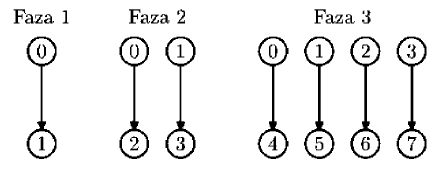
\includegraphics[width=0.8\textwidth]{./img/bcast.png}
	\caption{Schemat rozgłaszania dla 8 procesów. Źródło: \cite{Czech}, str 180}
	\label{img:sieć}
\end{figure} 
 
\subsubsection{MPI\textunderscore Reduce}

Funkcja redukcji również należy do komunikacji kolektywnej i stanowi przeciwieństwo rozgłaszania. Jest to operacja typu "wszystkie do jednego" (ang. \textit{all-to-one}). Nagłówek tej funkcji ma następującą postać:

\begin{lstlisting}[language=C]
int MPI_Reduce(
	void* collected_data,
	void* result_data,
	int count,
	MPI_Datatype type,
	MPI_Op operator,
	int dest,
	MPI_Comm comm);
\end{lstlisting}

Gdzie:

\begin{itemize}
	\item \texttt{\textbf{collected\textunderscore data}} -- adres pierwszej danej, na której zostanie wykonana operacja redukcji we wszystkich procesach w ramach komunikatora.
	\item \texttt{\textbf{result\textunderscore data}} -- adres pamięci, pod jaki zostanie zapisany wynik redukcji.
	\item \texttt{\textbf{count}} -- liczba danych, na których zostani wykonana operacja redukcji.
	\item \texttt{\textbf{type}} --  typ odbieranych i liczonych danych. Stanowi jeden z wbudowanych typów danych dla MPI \hyperref[table:datatypes]{Rozdział 2.5} lub typ pochodny zdefiniowany przez użytkownika.
	\item \texttt{\textbf{operator}} -- wskazuje, jaki rodzaj operacji ma zostać wykonany na odebranych danych.
	\item \texttt{\textbf{dest}} -- identyfikator wskazujący, który proces ma odebrać i przetworzyć dane.
	\item \texttt{\textbf{comm}} -- komunikator, w ramach którego wykonana zostanie operacja redukcji
\end{itemize}

\begin{figure}[h]
	\centering
	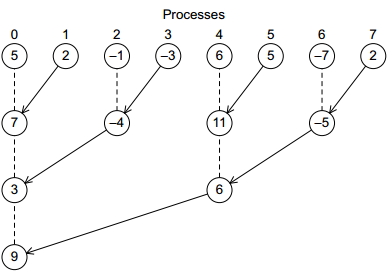
\includegraphics[width=0.6\textwidth]{./img/redukcja.png}
	\caption{Przykładowy schemat redukcji sumy dla 8 procesów. Źródło: \cite{Pacheco}, str 102}
	\label{img:sieć}
\end{figure}

Operacja redukcji polega na zredukowaniu danych lokalnych przechowywanych w procesach do jednej danej, charakteryzującej lokalnie zbiór danych. Po jej wykonaniu, wynik zostaje zapisany w procesie korzeniu. Niemal wszystkie parametry w funkcji \texttt{MPI\textunderscore Reduce} mają charakter wejściowy zarówo dla korzenia odbierającego dane jak i procesów wysyłających. Wyjątkiem jest parametr przechowujący informację o wyniku, mający charakter wyjściowy.

W tabeli \ref{table:reduceOp} przedstawiono dostępne operacje, które można wstawić w miejsce argumentu \texttt{operator}. Istnieje możliwość zadefiniowania własnej operacji redukcji. Większość standardowych operacji redukowana jest do pojedynczej wartości. Wyjątek od reguły stanowią \texttt{MPI\textunderscore MAXLOC} oraz \texttt{MPI\textunderscore MINLOC}, gdzie zarówno dane wyjściowe jak i wyjściowe stanowią parę wielkości. Parę wejściową tworzą dana podlegająca redukcji, a także identyfikator procesu, w którym ta dana się znajduje. Analogicznie, parę wyjściową stanowi dana wynikowa (maksimum lub minimum pośród danych lokalnych wszystkich węzłów) oraz numer jej procesu.

\begin{figure}[h]
	\begin{center}
	\begin{tabular}{|c|c|c|}
		\hline Nazwa & Znaczenie & Typ argumentów \\ 
		\hline MPI\textunderscore MAX & maksimum & całkowity oraz rzeczywisty \\ 
		\hline MPI\textunderscore MIN & minimum & całkowity oraz rzeczywisty \\ 
		\hline MPI\textunderscore SUM & suma & całkowity oraz rzeczywisty \\ 
		\hline MPI\textunderscore PROD & iloczyn & całkowity oraz rzeczywisty \\ 
		\hline MPI\textunderscore LAND & logiczne and & całkowity \\ 
		\hline MPI\textunderscore LOR & logiczne or & całkowity \\ 
		\hline MPI\textunderscore LXOR & logiczne exclusive or & całkowity \\ 
		\hline MPI\textunderscore BAND & bitowe and & całkowity oraz byte \\ 
		\hline MPI\textunderscore BOR & bitowe or & całkowity oraz byte \\ 
		\hline MPI\textunderscore BXOR & bitowe exclusive or & całkowity oraz byte \\ 
		\hline MPI\textunderscore MAXLOC & maksmum i jego lokalizacja & pary wielkości \\ 
		\hline MPI\textunderscore MINLOC & minimum i jego lokalizacja & pary wielkości \\ 
		\hline 
	\end{tabular} 
	\captionof{table}{Dostępne operacje dla funkcji MPI\textunderscore Reduce Źródło: \cite{MPI}, str 176} \label{table:reduceOp} 
	\end{center}
\end{figure}

\subsubsection{Dodatkowe funkcje i struktury}

Podobnie jak przypadku komunikacji typu punkt-punkt, do dyspozycji programisty zostały oddane inne funkcje umożliwiające komunikację kolektywną.

\begin{description}
	\item[\texttt{MPI\textunderscore Allreduce}] stanowi alternatywną wersję \texttt{MPI\textunderscore Reduce}. Posiada prawie identyczną listę argumentów, a jedyną różnicą jest brak argumentu numeru procesu docelowego. Wynika z założenia działania funkcji -- po dokonaniu redukcji, wynik działania wysyłany jest do wszystkich procesów w ramach komunikatora.
	\item[\texttt{MPI\textunderscore Scatter}] rozdziela dane zapisane w ciągłej struturze danych (np. tablicy) oraz przesyła je z pojedynczego procesu źródłowego do pozostałych procesów w ramach komunikatora. Proces źródłowy (korzeń) dzieli wektor danych na p (liczba procesów w komunikatorze biorących udział w obliczeniach) elementów i rozsyła je do pozostałych procesów (włącznie ze sobą samym). W wyniku takiej operacji, każdy proces otrzyma fragment danych do obliczeń. \texttt{MPI\textunderscore Scatter} wymaga od wszystkich procesów wcześniejszego zainicjalizowania dwóch tablic: jednej przechowującej adres wysyłanych danych oraz drugiej przechowującej adres pobranych danych.
	\item[\texttt{MPI\textunderscore Gather}] jest funkcją o działaniu odwrotnym do \texttt{MPI\textunderscore Scatter}. Jej wywołanie spowoduje zebranie danych ze wszystkich (w ramach komunikatora) przez procesor zwany korzeniem. Dane umieszczane są pamięci podręcznej korzenia wskazanej jednym z argumentów. Wszystkie pobrane porcje danych powinny być tej samej wielkości, o co dba wcześniej wywoływana funkcja \texttt{MPI\textunderscore Scatter}.
	\item[\texttt{MPI\textunderscore Comm\textunderscore split}] jest funkcją wywoływaną przez wszystkie procesy w ramach komunikatora. Efektem wywołania jest podział starego komunikatora na nowy według określonego klucza. Zadaniem funkcji jest ułatwienie grupowania procesów.
\end{description}
